% TikZ Architecture Diagram for lix_cache
% Standalone file — can be \input{} into main paper or compiled separately
\documentclass[border=10pt]{standalone}
\usepackage{tikz}
\usetikzlibrary{positioning, arrows.meta, shapes.geometric, fit, calc, decorations.pathreplacing}

\begin{document}
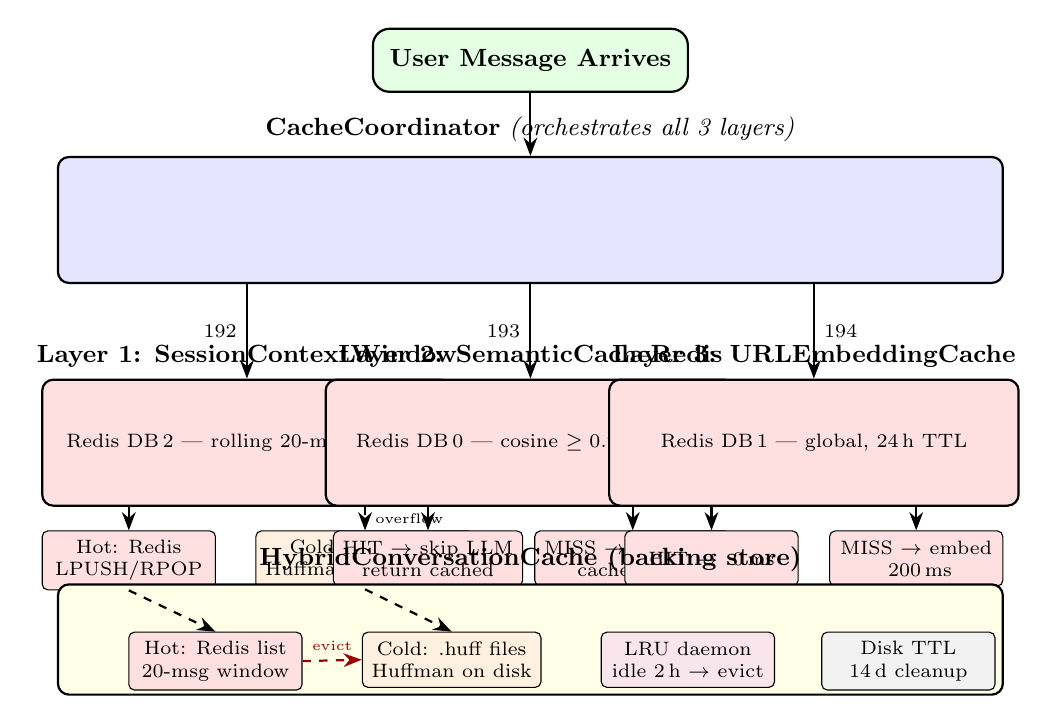
\begin{tikzpicture}[
    node distance=0.8cm and 1.2cm,
    >=Stealth,
    every node/.style={font=\small},
    layer/.style={draw, rounded corners=4pt, minimum width=5.2cm, minimum height=1.6cm, align=center, thick},
    sublayer/.style={draw, rounded corners=2pt, minimum width=2.2cm, minimum height=0.7cm, align=center, font=\scriptsize, thin},
    redis/.style={fill=red!12},
    disk/.style={fill=orange!12},
    coord/.style={fill=blue!10},
    arrow/.style={->, thick, >=Stealth},
    dasharrow/.style={->, thick, dashed, >=Stealth},
    brace/.style={decorate, decoration={brace, amplitude=6pt, raise=2pt}},
]

% ── User message ──
\node[draw, rounded corners=6pt, fill=green!10, minimum width=4cm, minimum height=0.8cm, thick]
    (user) {\textbf{User Message Arrives}};

% ── CacheCoordinator ──
\node[layer, coord, below=0.8cm of user, minimum width=12cm]
    (coordinator) {};
\node[above=0.05cm] at (coordinator.north) {\textbf{CacheCoordinator} \textit{(orchestrates all 3 layers)}};

% ── Layer 1: Session Context Window ──
\node[layer, redis, below=1.2cm of coordinator.south west, anchor=north west, xshift=-0.2cm]
    (session) {};
\node[above=0.02cm, font=\small\bfseries] at (session.north) {Layer 1: SessionContextWindow};
\node[font=\scriptsize] at (session.center) {Redis DB\,2 — rolling 20-msg window};

\node[sublayer, redis, below=0.3cm of session.south, xshift=-1.5cm]
    (hot) {Hot: Redis\\LPUSH/RPOP};
\node[sublayer, disk, below=0.3cm of session.south, xshift=1.5cm]
    (cold) {Cold: .huff disk\\Huffman compressed};

% ── Layer 2: Semantic Query Cache ──
\node[layer, redis, below=1.2cm of coordinator.south, anchor=north]
    (semantic) {};
\node[above=0.02cm, font=\small\bfseries] at (semantic.north) {Layer 2: SemanticCacheRedis};
\node[font=\scriptsize] at (semantic.center) {Redis DB\,0 — cosine $\geq 0.90 \Rightarrow$ HIT};

\node[sublayer, redis, below=0.3cm of semantic.south, xshift=-1.3cm]
    (semhit) {HIT $\rightarrow$ skip LLM\\return cached};
\node[sublayer, redis, below=0.3cm of semantic.south, xshift=1.3cm]
    (semmiss) {MISS $\rightarrow$ call LLM\\cache 5\,min};

% ── Layer 3: URL Embedding Cache ──
\node[layer, redis, below=1.2cm of coordinator.south east, anchor=north east, xshift=0.2cm]
    (urlcache) {};
\node[above=0.02cm, font=\small\bfseries] at (urlcache.north) {Layer 3: URLEmbeddingCache};
\node[font=\scriptsize] at (urlcache.center) {Redis DB\,1 — global, 24\,h TTL};

\node[sublayer, redis, below=0.3cm of urlcache.south, xshift=-1.3cm]
    (urlhit) {HIT $\rightarrow$ ~0\,ms};
\node[sublayer, redis, below=0.3cm of urlcache.south, xshift=1.3cm]
    (urlmiss) {MISS $\rightarrow$ embed\\~200\,ms};

% ── HybridConversationCache backing store ──
\node[draw, rounded corners=4pt, fill=yellow!10, minimum width=12cm, minimum height=1.4cm, thick,
      below=3.8cm of coordinator.south, anchor=north]
    (hybrid) {};
\node[above=0.02cm, font=\small\bfseries] at (hybrid.north) {HybridConversationCache (backing store)};

\node[sublayer, redis, below=-0.1cm of hybrid.center, xshift=-4cm]
    (hybhot) {Hot: Redis list\\20-msg window};
\node[sublayer, disk, below=-0.1cm of hybrid.center, xshift=-1cm]
    (hybcold) {Cold: .huff files\\Huffman on disk};
\node[sublayer, fill=purple!10, below=-0.1cm of hybrid.center, xshift=2cm]
    (hyblru) {LRU daemon\\idle 2\,h $\rightarrow$ evict};
\node[sublayer, fill=gray!10, below=-0.1cm of hybrid.center, xshift=4.8cm]
    (hybttl) {Disk TTL\\14\,d cleanup};

% ── Arrows: user → coordinator ──
\draw[arrow] (user.south) -- (coordinator.north);

% ── Arrows: coordinator → layers ──
\draw[arrow] (coordinator.south -| session.north) -- (session.north)
    node[midway, left, font=\scriptsize] {\ding{192}};
\draw[arrow] (coordinator.south) -- (semantic.north)
    node[midway, left, font=\scriptsize] {\ding{193}};
\draw[arrow] (coordinator.south -| urlcache.north) -- (urlcache.north)
    node[midway, right, font=\scriptsize] {\ding{194}};

% ── Arrows: session → hot/cold ──
\draw[arrow] (session.south -| hot.north) -- (hot.north);
\draw[dasharrow] (session.south -| cold.north) -- (cold.north)
    node[midway, right, font=\tiny] {overflow};

% ── Arrows: semantic → hit/miss ──
\draw[arrow] (semantic.south -| semhit.north) -- (semhit.north);
\draw[arrow] (semantic.south -| semmiss.north) -- (semmiss.north);

% ── Arrows: url → hit/miss ──
\draw[arrow] (urlcache.south -| urlhit.north) -- (urlhit.north);
\draw[arrow] (urlcache.south -| urlmiss.north) -- (urlmiss.north);

% ── Arrows: hot/cold → hybrid ──
\draw[dasharrow] (hot.south) -- (hybhot.north);
\draw[dasharrow] (cold.south) -- (hybcold.north);

% ── LRU arrow ──
\draw[dasharrow, red!60!black] (hybhot.east) -- (hybcold.west)
    node[midway, above, font=\tiny, red!60!black] {evict};

\end{tikzpicture}
\end{document}
